% Use only LaTeX2e, calling the article.cls class and 12-point type.

\documentclass[12pt]{article}


% Users of the {thebibliography} environment or BibTeX should use the
% scicite.sty package, downloadable from *Science* at
% www.sciencemag.org/about/authors/prep/TeX_help/ .
% This package should properly format in-text
% reference calls and reference-list numbers.

\usepackage[super]{scicite}

% Use times if you have the font installed; otherwise, comment out the
% following line.

\usepackage{times}
\usepackage{graphicx}
\usepackage{caption} % removes colon after empty caption


% The preamble here sets up a lot of new/revised commands and
% environments.  It's annoying, but please do *not* try to strip these
% out into a separate .sty file (which could lead to the loss of some
% information when we convert the file to other formats).  Instead, keep
% them in the preamble of your main LaTeX source file.


% The following parameters seem to provide a reasonable page setup.
\topmargin 0.0cm
\oddsidemargin 0.2cm
\textwidth 16cm 
\textheight 21cm
\footskip 1.0cm


%The next command sets up an environment for the abstract to your paper.

\newenvironment{sciabstract}{%
\begin{quote} \bf}
{\end{quote}}


% If your reference list includes text notes as well as references,
% include the following line; otherwise, comment it out.

\renewcommand\refname{References and Notes}

% The following lines set up an environment for the last note in the
% reference list, which commonly includes acknowledgments of funding,
% help, etc.  It's intended for users of BibTeX or the {thebibliography}
% environment.  Users who ae hand-coding their references at the end
% using a list environment such as {enumerate} can simply add another
% item at the end, and it will be numbered automatically.

\newcounter{lastnote}
\newenvironment{scilastnote}{%
\setcounter{lastnote}{\value{enumiv}}%
\addtocounter{lastnote}{+1}%
\begin{list}%
{\arabic{lastnote}.}
{\setlength{\leftmargin}{.22in}}
{\setlength{\labelsep}{.5em}}}
{\end{list}}


% Include your paper's title here

\title{The length of words reflects their conceptual complexity}


% Place the author information here.  Please hand-code the contact
% information and notecalls; do *not* use \footnote commands.  Let the
% author contact information appear immediately below the author names
% as shown.  We would also prefer that you don't change the type-size
% settings shown here.

\author
{Molly L. Lewis and Michael C. Frank\\
\\
\normalsize{Psychology Department, Stanford University,}\\
\normalsize{450 Serra Mall, Stanford, CA 94305, USA}\\
\\
\normalsize{$^\ast$To whom correspondence should be addressed; E-mail: mll@stanford.edu.}
}


% Include the date command, but leave its argument blank.

\date{}

%%%%%%%%%%%%%%%%% END OF PREAMBLE %%%%%%%%%%%%%%%%
\begin{document} 

% Double-space the manuscript.
\baselineskip24pt

% Make the title.
\maketitle 

% Place your abstract within the special {sciabstract} environment.

% \begin{sciabstract}		

% \end{sciabstract}					

{\bf Are the forms of words systematically related to their meaning? The arbitrariness of the sign has long been a foundational part of our understanding of human language \cite{saussure,hockett1960}. Theories of communication predict another relationship between form and meaning, however: Longer descriptions should convey more complex meanings \cite{horn1984,jaeger2006}. Here we show that both the lexicons of human languages and individual speakers encode the relationship between linguistic and cognitive complexity. Experimentally, participants mapped longer words to more complex objects in comprehension and production tasks and across a range of stimuli. Explicit judgments of complexity were also highly correlated with implicit measures of study time in a memory task, suggesting that complexity is directly related to basic cognitive processes. Observationally, judgements of complexity for a sample of real words correlate highly with their length across 80 languages, even controlling for frequency, familiarity, imageability, and concreteness. These results point to a general regularity in the design of lexicons and suggest the importance of communicative and cognitive constraints on language evolution \cite{christiansen2008,lieberman2007}.}


In a classic example of pragmatic reasoning \cite{horn1984}, the utterance ``Lee got the car to stop'' seems to imply an unusual state of affairs. Had the speaker wished to convey that Lee simply applied the brakes, the shorter and less exceptional ``Lee stopped the car'' would be a better description. The use of a longer utterance licenses the inference that there was some problem in stopping---perhaps the brakes failed---and that the situation is more complex. Does this same reasoning apply to the meanings of words? Is a ``tupabugorn'' more likely to be a complex, unusual object than a ``bugorn''? 

\begin{figure}[t]
\begin{center}
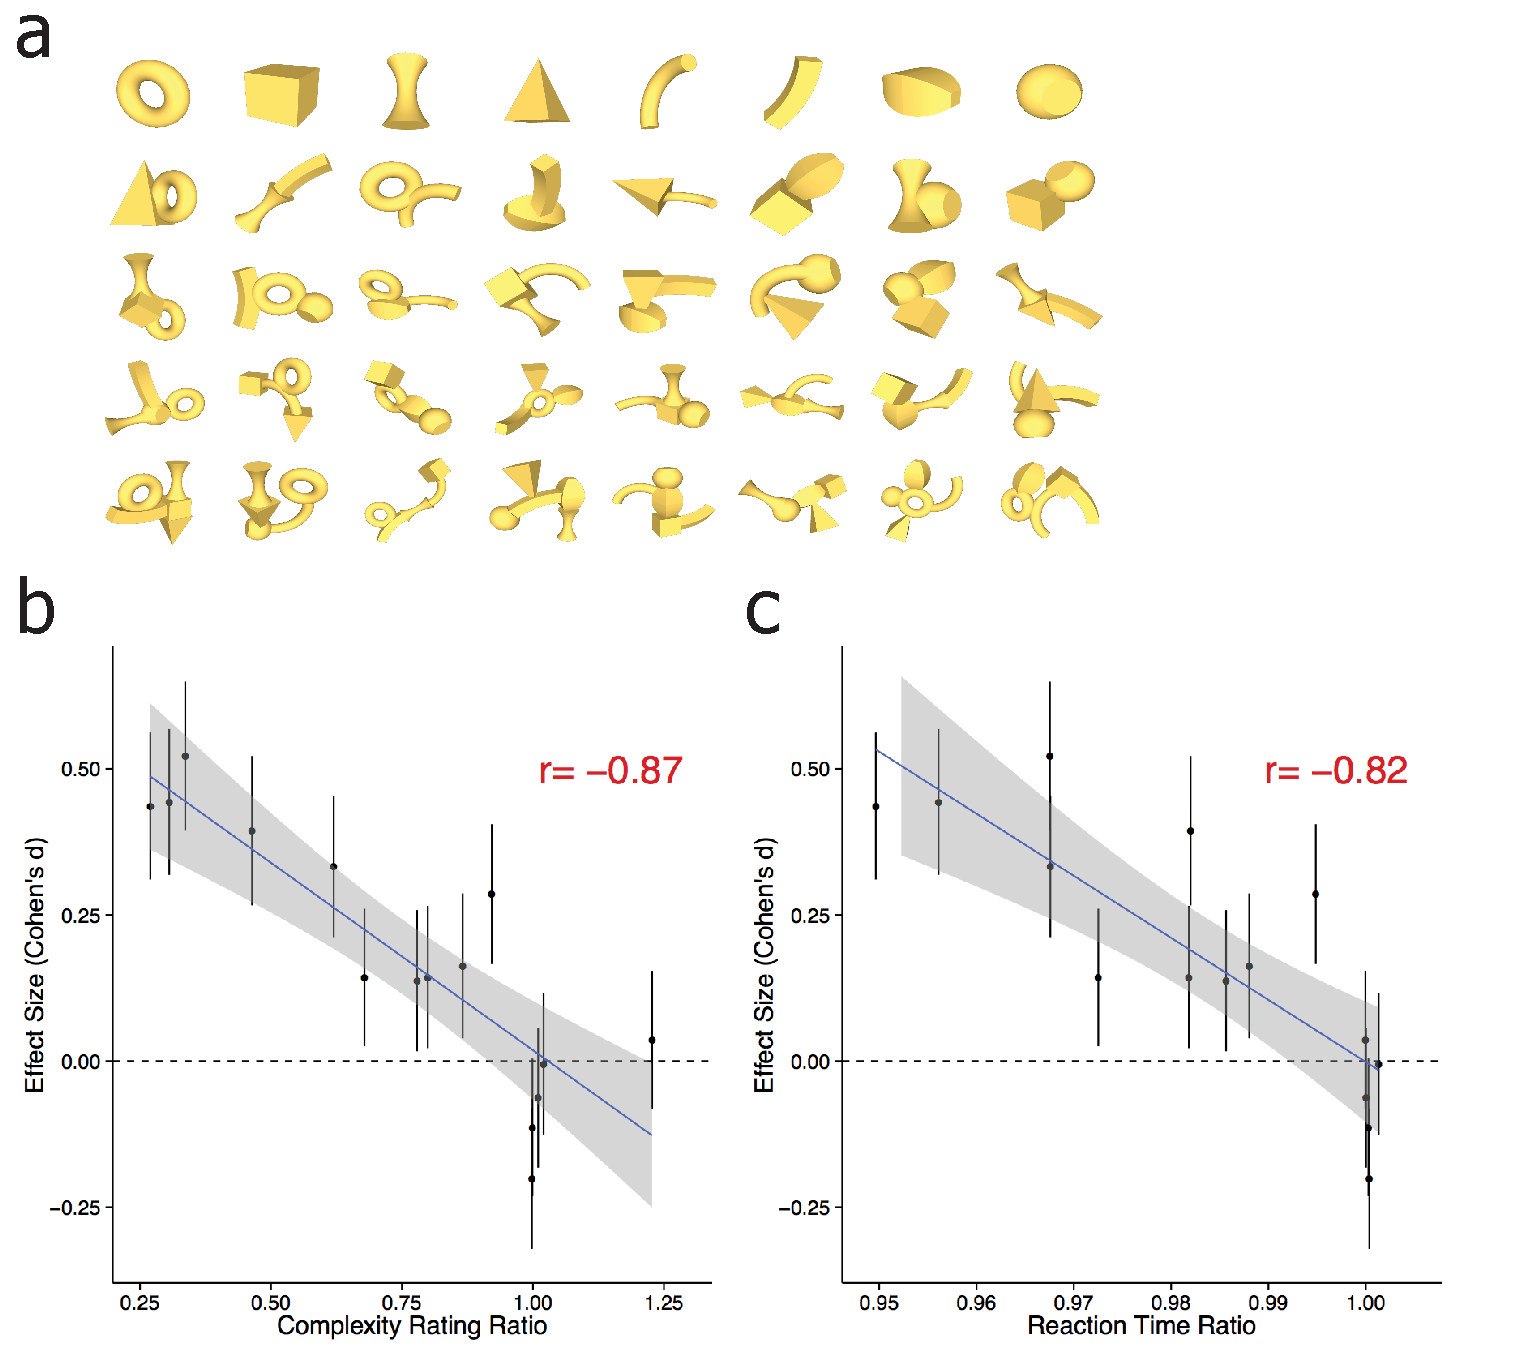
\includegraphics[scale = .5]{figs/geons.pdf}
\caption{}
\end{center}
\label{fig:geons}
\end{figure}

We tested this hypothesis by asking whether speakers would be biased to interpret a long novel word as being more likely to refer to a more complex novel referent. We presented participants on Amazon Mechanical Turk (Study 1: $N=750$) with a novel word of either 2 or 4 syllables and two possible objects as referents. Possible referents were novel artificial objects whose complexity we manipulated by varying the number of parts the object contained (1 - 5 ``geons'' \cite{biederman1987}; Fig.\ 1a; these judgements were highly correlated with explicit complexity judgments, Study 2: $r = .93$, $p < .0001$). Participants were asked to select which object the word named for every unique combination of object complexities (1 vs.\ 2 geons, 1 vs.\ 3 geons, 1 vs.\ 4 geons, etc.).

Across conditions, the more complex object was more likely to be judged the referent of the longer word. For each condition (e.g., 1 vs.\ 2 geons), we calculated the effect size for participants' complexity bias---the degree to which the complex object was more likely to be chosen as the referent of a long word, compared to the short word.  Effect size was highly correlated with the ratio of object complexities: The greater the mismatch in object complexity, the more the longer word was paired with the more complex object ($r = -.87$, $p < .0001$; Fig.\ 1b). In a control experiment, we also found this bias with words that were composed of randomly concatenated syllables: participants were more likely to select a five geon object compared to a single geon object as the number of syllables in the word increased (Study 3: $N=200$; $\beta=-.44$, $p <.0001$).
					
\begin{figure}[t]
\begin{center}
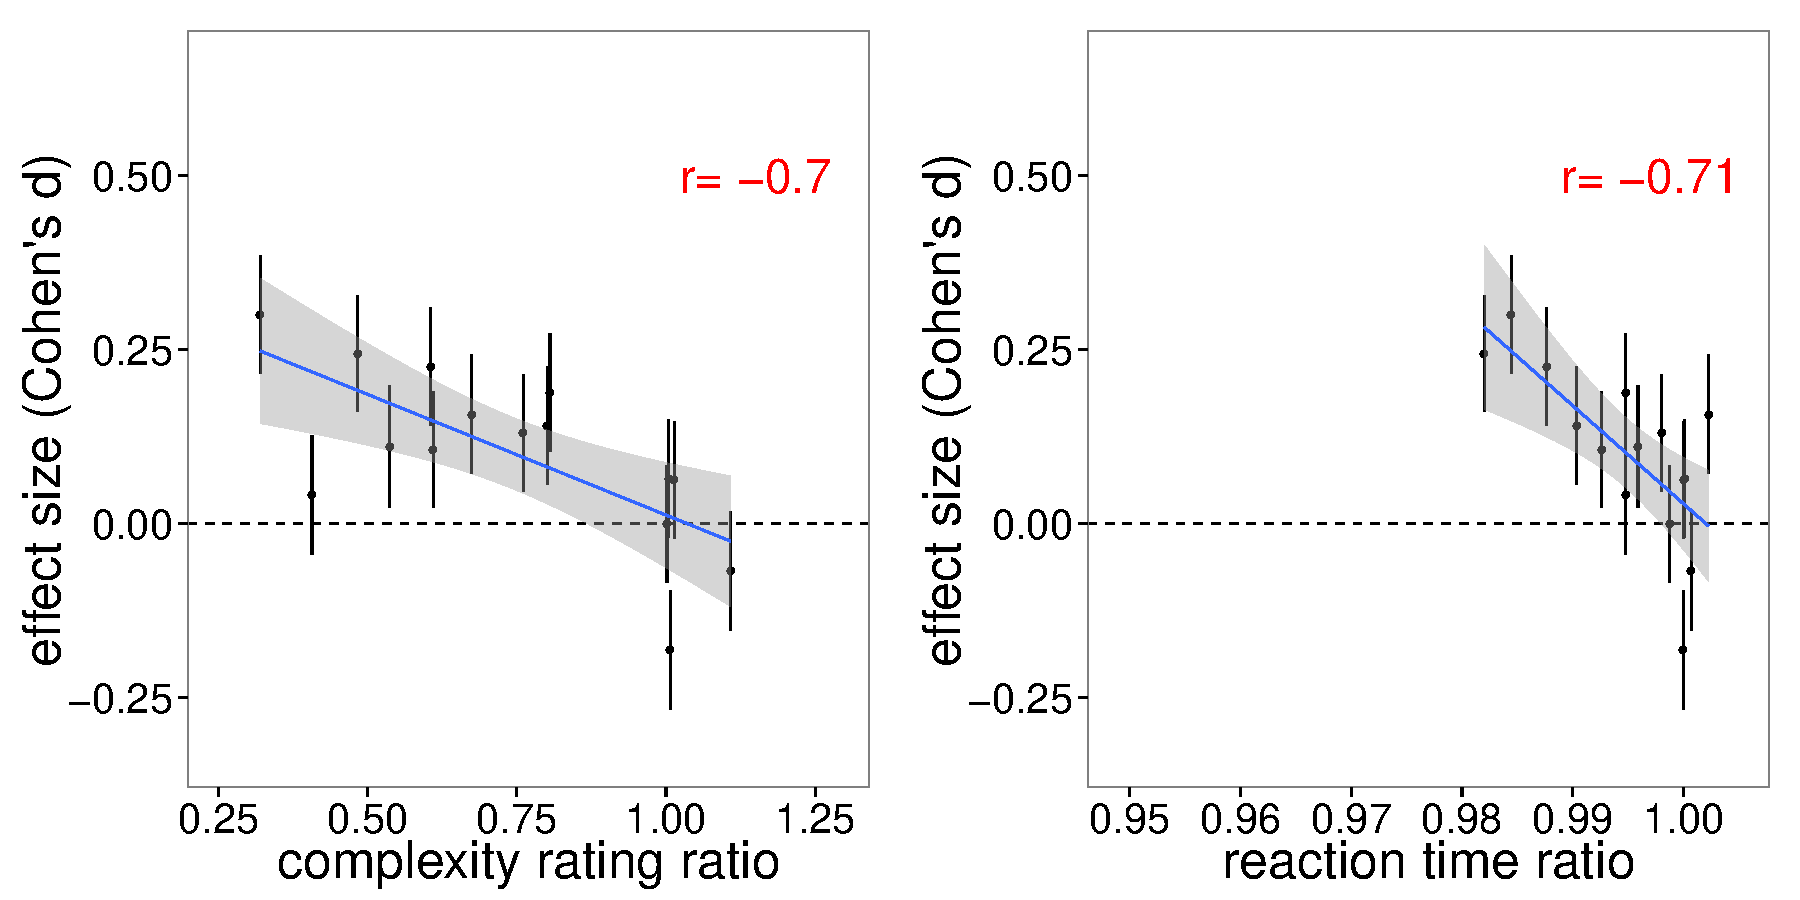
\includegraphics[scale = .5]{figs/realobjs.pdf}
\caption{}
\end{center}
\label{fig:real_objs}
\end{figure}

Next we asked whether this bias extended to more naturalistic objects. We gathered a sample of real objects without canonical labels (Fig.\ 2a) and asked participants to rate their complexity. These judgements were highly reliable across two independent samples (Study 4: N = 60 in each, $r = .93$, $p < .0001$). We then divided the objects into quintiles based on these ratings, and used them as stimuli in a mapping task identical to the one used with the artificial objects. As with the artificial objects, effect size was negatively correlated with the complexity judgment ratio between the referent alternatives (Study 5: $N = 1500$; $r = .70$, $p < .005$; Fig.\ 2b). We also replicated this result with randomly concatenated syllables, such that participants were more likely to select an object from the fifth quintile as opposed to the first quintile when the novel word contained more syllables (Study 6: $N=200$, $\beta=-.34,$ $p <.0001$). Finally, we  also found the same bias in language production: Participants produced novel coinages that were longer for the top quartile of objects compared to the bottom quartile (Study 7: $N=59$; $t(57) = 3.92$, $p < .001$). 
					
If complexity is related to a basic cognitive process, we should be able to measure it using an implicit task, not just via explicit ratings. In visual cognition, stimuli that contain more information require more processing time in search \cite{alvarez2004capacity, hyman}. To test this prediction, we measured participants' study time of objects in a memory task. Each participant studied half of the objects in the stimulus set, one at a time, and then made old/new judgments for the entire set. Critically, the study phase was self-paced, such that participants were allowed to study each object for as much time as they wanted. This study time provided an implicit measure of complexity.
					
Mean study time was highly correlated with explicit complexity norms for both artificial objects (Study 8: $N = 250$; $r = .89$, $p < .0001$) and novel real objects (Study 9: $N = 500$; $r = .54$, $p < .0001$). In addition, the ratio of study times for the two object alternatives was correlated with the bias to choose a longer label for both the artificial objects ($r = .82$, $p < .001$; Fig.\ 1c) and the novel real objects ($r = .71$, $p < .005$; Fig.\ 2c): Relatively longer study times predicted longer labels. These findings suggest that label judgments are supported by basic cognitive processes related to the complexity or information content of a stimulus. 
					
Together, these experiments point to a complexity bias in interpreting novel labels: Words that are longer tend to be associated with meanings that are more complex, as reflected in both explicit and implicit measures. Is this bias only relevant to judgments of unfamiliar words, or does it apply to familiar labels as well? 

\begin{figure}[t]
\begin{center}

\includegraphics[scale = .53]{figs/xling.pdf}
\caption{} 
\end{center}
\label{fig:real_objs}
\end{figure}

We collected ratings of meaning complexity for 499 English words (Study 10: $N = 250$). Longer English words had meanings that were rated as more complex in a rating procedure similar to Studies 2 and 4. Complexity judgements were positively correlated with word length, measured in syllables, phonemes, and morphemes ($r_{syllables} = .63$, $r_{phonemes} = .66$, $r_{morphemes} = .43$, all $p$s $< .0001$), even when closed-class words were excluded ($N = 453$; $r_{syllables} = .62$, $r_{phonemes} = .66$, $r_{morphemes} = .43$, all $p$s $< .0001$). Importantly, these relationships also remained reliable after controlling for the word's concreteness, imageability, and familiarity. 
						
If the complexity bias relies on a universal cognitive process, it should generalize to lexicons beyond English. We explored this prediction in 79 additional languages, using Google Translate to translate our word set (Study 11). Native speakers checked the accuracy of these translations for 12 of the 79 languages, finding an accuracy of .92 within this sample. For each language, we calculated the correlation between word length in terms of number of characters (to allow comparison between languages for which no phonetic dictionary was available) and mean complexity rating. All 79 languages showed a positive correlation between length and complexity ratings (Fig. 3). The grand mean correlation across languages was .34. 
					
Word length is also strongly related to linguistic predictability, operationalized via simple frequency \cite{zipf1936} or using a language model \cite{piantadosi2011a}. But the regularity we describe---a relationship between conceptual complexity and word length---holds even when controlling for frequency. In English, the correlation was only slightly reduced when controlling for log frequency ($r = .56$, $p < .0001$). Across languages, partialling out log frequency (estimated in English), the grand mean correlation was .22. In addition, in a number of experiments, when we manipulated the observed frequencies of novel objects, we found no effects on judgments of word length (Studies 12--13). 

Languages also show phonological iconicity effects, such that semantic features \cite{maurer2006shape} and even particular form classes \cite{farmer2006phonological} are marked by particular sound patterns. Our findings could be due to some broad iconic relationship between abstract measures of complexity and amount of verbal or orthographic effort---indeed this is precisely the relationship that Horn originally noticed. But specific iconic hypotheses that posit a parallel between an object's parts and the number of phonemes, morphemes, or syllables in its label do not account for the patterns in the English lexicon, which hold for monomorphemic words alone ($N = 387$; $r_{syllables} = .46$, $r_{phonemes} = .53$, all $p$s $< .0001$) and for abstract ideas that have no obvious part structure ($r = .75$, $p< .0001$, for the 249 least concrete nouns). 

What are the origins of structure in human language? Our findings reveal a broad systematicity in the design of  languages---a bias for longer words to map to more complex meanings---and suggest that properties of the human cognitive system may underly this systematicity. We find that referents that contain more information, and consequently take longer for the cognitive system to process (as measured by study time), tend to be associated with longer labels. This broad systematicity both within and across languages fundamentally challenges the assumption that lexicons are arbitrary, and suggests that the structure of the lexicon reflects a basic communicative bias to associate longer forms with meanings containing more information.


\paragraph*{Methods}
All participants in the experimental studies were recruited on Amazon Mechanical Turk and paid \$0.15-0.30 for their participation, depending on the length of the task. 

In Studies 1 and 5, we manipulated word length (2 vs.\ 4 syllables) and the relative complexity of the referent alternatives within participants.  There were 15 complexity conditions, corresponding to every possible combination of object quintiles. In Study 1, the quintiles were determined by the number of geons in the object. In Study 5, the quintiles were determined by the norms obtained in Study 4. Each participant completed 4 short and 4 long trials in a random order, where each word was randomly associated with one of the complexity conditions. No participant saw the same complexity condition twice and no word or object was repeated across trials. 

In Studies 2 and 4, we presented participants with 12 objects from the the full stimulus set one at a time. For each object, we asked ``How complicated is this object?,'' and participants responded using a slider scale, anchored at ``simple'' and ``complicated.'' The first two objects were an image of a ball and a motherboard to anchor participants on the scale.

In the Studies 3 and 6,  participants completed six forced-choice trials in which they saw two possible referents, from the top and bottom quintiles. The novel words were created by randomly concatenating 2, 4, or 6 consonant-vowel syllables. The last syllable of all words ended in a consonant. Each participant completed 2 trials for each word length. 

In Study 7, participants were presented 10 objects from the set of objects normed in Study 4 and asked to generate a novel single-word label for the object. Five of the objects were from the bottom quantile of complexity norms, and 5 of the objects were from the top quantile of complexity norms. Order of objects was randomized.

In Studies 8 and 9, participants were told they were going to view some objects and their memory of those exact objects would later be tested. In the study phase, participants were presented with half of the full stimulus set one at a time (20 geon objects and 30 naturalistic objects) and allowed to click a ``next'' button when they were done studying each object. After the training phase, we presented participants with each object in the full stimulus set  (40 geon object and 60 naturalistic objects), and asked ``Have you seen this object before?.'' Participants responded by clicking a ``yes'' or ``no'' button.

In Study 10, we selected 499 relatively high-frequency English words that were included in the MRC corpus. For each word, we asked ``How complex is the meaning of this word?," and participants indicated their response on a 7-pt Likert scale, anchored at ``simple" and ``complex." Each participant rated 30 words.

In Study 12 (N = 477), we presented participants with 10 objects on a single screen. The objects were composed of a single geon. There were two different types of objects. One object type appeared nine times (``high frequency object") and the second object type appeared once (``low frequency object"). After this training period, participants completed a forced choice mapping task, as in Studies 1 and 5. We presented a word that was either 2 or 4 syllables long and asked participants to make a judgment about whether the word referred to the low or high frequency object. Each participant completed a single mapping trial, and word length was manipulated between participants. There was no difference between the long and short word conditions ($\chi ^2(1) = 0.02$,  $p = .89$).

In Study 13 (N = 97), we manipulated object frequency by sequentially presenting objects. Participants saw 60 objects from the  set of normed real objects one at a time. One object was presented 10 times and a second object was presented 40 times. Ten additional objects were included as fillers. After this training phase, participants completed a single mapping trial as in Study 12. Word length was manipulated between participants. There was no difference between the long and short word conditions ($\chi ^2(1) = 0.01$,  $p = .92$).

\renewcommand{\refname}{\normalsize References}
\bibliography{biblibrary}
\bibliographystyle{Science}

\paragraph*{Supplementary Information}

\paragraph*{Acknowledgements}

\paragraph*{Author Contributions}

\paragraph*{Author Information}

\paragraph*{Figure Legends}~ \\

\noindent {\it Figure 1.} Artificial ``geon" stimuli. Each row shows a different level of complexity, determined by the number of geon parts in the objects. (b, c) Experimental results from task in which participants were asked to map a novel word of varying length to one of two possible referents. Effect size between the long and short language conditions is plotted against the complexity ratio of the two referent alternatives. Fig.\ 1b shows the referents plotted in terms of explicit complexity judgements, and Fig.\ 1c shows the referents plotted in terms of reaction time. Error bars show 95\% confidence intervals.
 \\
 \\
  {\it Figure 2.} (a) Naturalistic, novel stimuli. Each row corresponds to a quintile determined by the explicit complexity judgements (top: least complex; bottom: most complex). (b, c) Experimental results from task in which participants were asked to map a novel word of varying length to one of two possible referents. Effect size between the long and short language conditions is plotted against the complexity ratio of the two referent alternatives. Fig.\ 2b shows the referents plotted in terms of explicit complexity judgements, and Fig.\ 2c shows the referents plotted in terms of reaction time. Error bars show 95\% confidence intervals.
  \\
  \\ 
 {\it Figure 3.}  Correlations between conceptual complexity norms and word lengths, across languages. Dark red bars indicate languages for which translations were checked by native speakers; all other bars show translations obtained via Google Translate. Error bars show 95\% confidence intervals obtained via non-parametric bootstrap. Triangles indicate correlation value partialling out English log frequency. The dashed line indicates the grand mean correlation across languages.


% Following is a new environment, {scilastnote}, that's defined in the
% preamble and that allows authors to add a reference at the end of the
% list that's not signaled in the text; such references are used in
% *Science* for acknowledgments of funding, help, etc.



% For your review copy (i.e., the file you initially send in for
% evaluation), you can use the {figure} environment and the
% \includegraphics command to stream your figures into the text, placing
% all figures at the end.  For the final, revised manuscript for
% acceptance and production, however, PostScript or other graphics
% should not be streamed into your compliled file.  Instead, set
% captions as simple paragraphs (with a \noindent tag), setting them
% off from the rest of the text with a \clearpage as shown  below, and
% submit figures as separate files according to the Art Department's
% instructions.

%Our findings point to a previously undescribed regularity in the design of human languages --- a bias for longer words to map to more complex meanings.  This bias is found in both novel judgements about word meanings and in the structure of real lexicons. Importantly, the notion of complexity underlying this systematicity appears to be related to a basic cognitive process (as indexed by reaction time), suggesting that properties of the cognitive system may play a role in shaping the structure of language. More generally, our results reveal a broad systematicity between form and meaning in language that fundamentally challenges the long held assumption that lexicons are arbitrary.


\clearpage

\end{document}


